\chapter{Результаты}\label{ch:results}
В ходе работы были посчитаны деформации модели для следующих конфигураций:

Для упрощение представления результатов заменим реальные значения физ величин эквивалентным, при условии $E=10$.

Введём обозначения
\begin{gather*}
    \lambda - линейная плотность утка и основы в нитях на см \\
    A - амплитудный множитель силы удара \\
    r - радиус области удара
\end{gather*}

\begin{figure}[H]
    \centering
    \caption{$\lambda=1~нитей/см,~r=1~см,~A=0.1$}

    \begin{subfigure}[t]{0.5\textwidth}
        \centering
        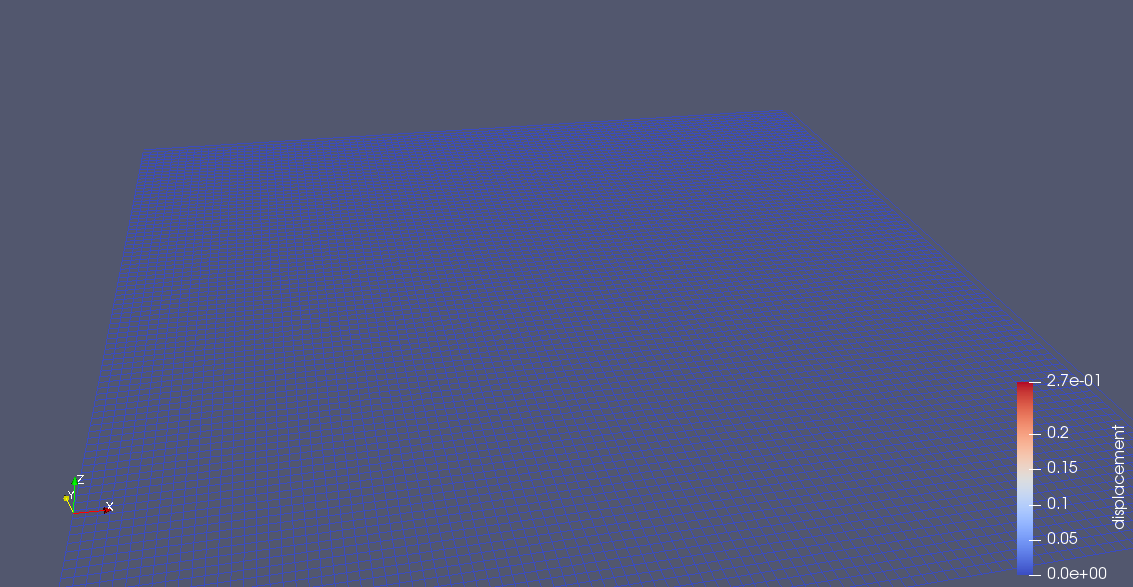
\includegraphics[width=\textwidth]{img/fiber/density_1_radius_1_amplitude_0.1/1.png}
    \end{subfigure}%
    ~
    \begin{subfigure}[t]{0.5\textwidth}
        \centering
        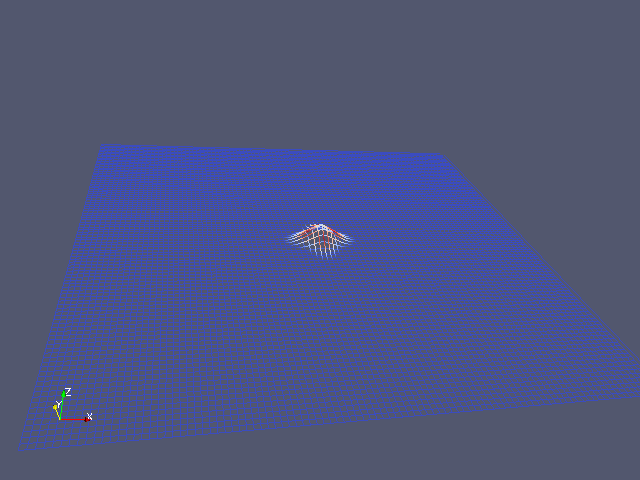
\includegraphics[width=\textwidth]{img/fiber/density_1_radius_1_amplitude_0.1/2.png}
    \end{subfigure}
    ~
    \begin{subfigure}[t]{0.5\textwidth}
        \centering
        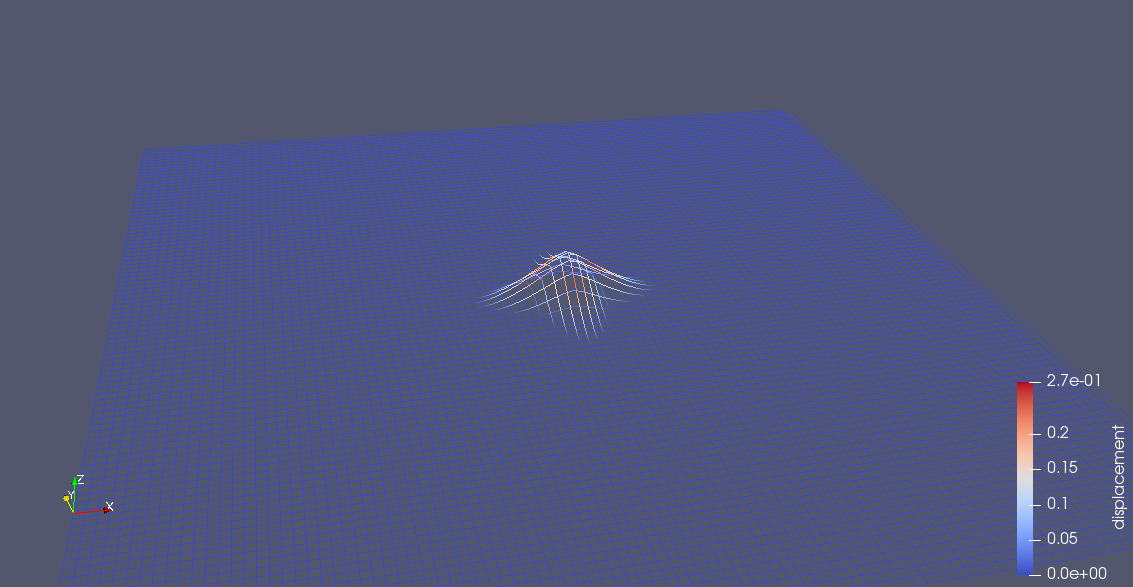
\includegraphics[width=\textwidth]{img/fiber/density_1_radius_1_amplitude_0.1/3.png}
    \end{subfigure}%
    ~
    \begin{subfigure}[t]{0.5\textwidth}
        \centering
        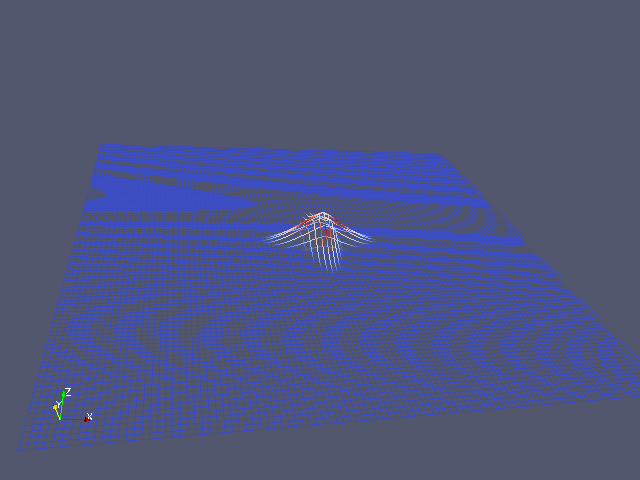
\includegraphics[width=\textwidth]{img/fiber/density_1_radius_1_amplitude_0.1/4.png}
    \end{subfigure}
    ~
    \begin{subfigure}[t]{0.5\textwidth}
        \centering
        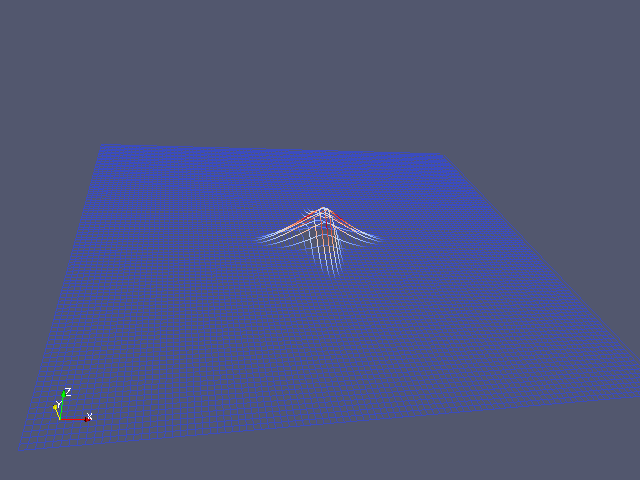
\includegraphics[width=\textwidth]{img/fiber/density_1_radius_1_amplitude_0.1/5.png}
    \end{subfigure}%
    ~
    \begin{subfigure}[t]{0.5\textwidth}
        \centering
        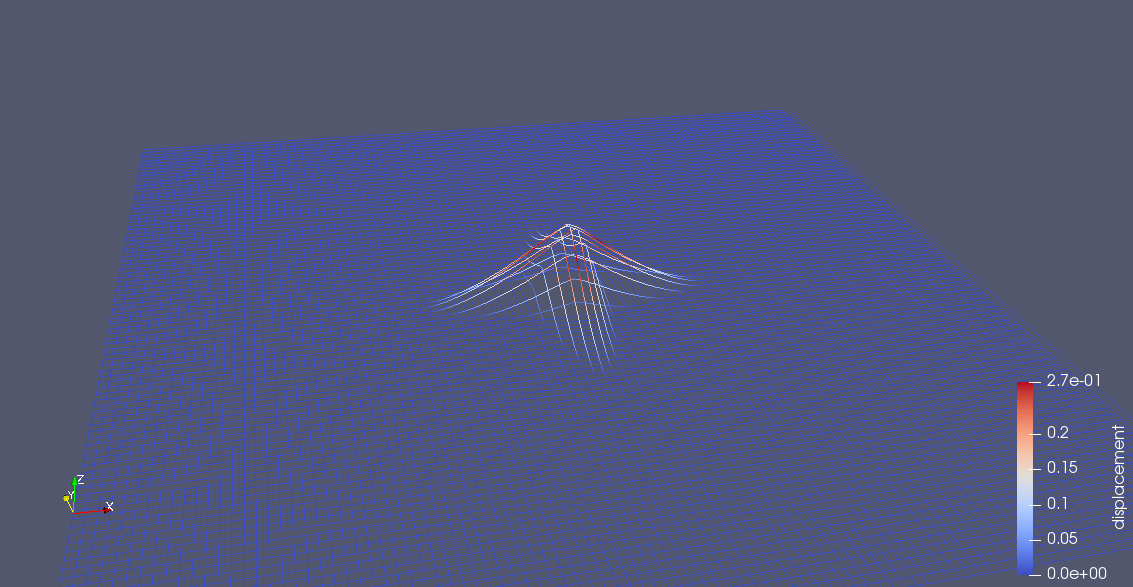
\includegraphics[width=\textwidth]{img/fiber/density_1_radius_1_amplitude_0.1/6.png}
    \end{subfigure}
\end{figure}
